%----------------------------------------------------------------------------------------
%	DOCUMENT CONFIGURATIONS
%----------------------------------------------------------------------------------------
\documentclass[11pt]{article}

\usepackage{float}
\usepackage{caption}
\usepackage{subcaption}

\RequirePackage{amsmath}
\RequirePackage{amssymb}
\RequirePackage{amsthm}
\usepackage{amsfonts}
\usepackage{mathtools}

\usepackage{epsfig}
\usepackage{amscd}
\usepackage{graphicx}% Include figure files
\usepackage{dcolumn}% Align table columns on decimal point
\usepackage{bm}% bold math
\usepackage{enumerate}
\usepackage{tikz}


\usepackage[top=1.5in,bottom=1.5in,right=1.5in, left=1.5in]{geometry}

%----------------------------------------------------------------------------------------
%	TITLE SECTION
%----------------------------------------------------------------------------------------



%----------------------------------------------------------------------------------------
%	ARTICLE SECTION
%----------------------------------------------------------------------------------------

\begin{document}

\author{Meilei Jiang\\
    Department of Statistics and Operations Research\\
		University of North Carolina at Chapel Hill}
\title{Simulation study: Modified SVA versus SVA}

\maketitle
\section{Modified SVA}
In your papers \cite{leek2007capturing, leek2008general, leek2012sva}, you proposed a factor model for the relationship between expression values, measured biological factors and unmeasured biological and non-biological factors:
$$ \begin{aligned}
X = B S + \Gamma G + U
\end{aligned}$$
In order to remove the batch effects, you proposed SVA on the data set to estimate $G$. An essential idea of SVA is to identify a subset of genes (tests) which are strongly associated with unmeasured confounders, but not with the group outcome. Especially, an empirical bayesian approach has been applied to estimate the probabilities 
$$\begin{aligned}\pi_{i w} &= \text{Pr}(b_i = \vec{0} \text{ } \& \text{ } \gamma_i \neq \vec{0} | X, S, \hat{G}) \\
&= \text{Pr}(b_i = \vec{0} | \gamma_i \neq \vec{0}, X, S, \hat{G}) \text{Pr}( \gamma_i \neq \vec{0}| X, S, \hat{G})                      
\end{aligned}$$
Then use $\pi_{i w}$ to weight the $i$th row of $X$ and perform a singular value decomposition of the weighted $X$ to reconstruct $\hat{G}$.


However, if we estimate $\hat{G}$ in this approach, IRW-SVA, I think it assumes there exists such subset of genes (tests) in the data set. When such subset of genes (tests) does not exist, IRW-SVA could fail. I think there is an easy way to overcome this problem: 

we only need to estimate the probability $\pi_{i \gamma}$ to weight the $i$th row of residual matrix $R = X - \hat{B} S$. Then reconstruct $\hat{G}$ through the singular value decomposition of the weighted $R$.

In order to check this idea, I set up a simple simulation study to look at the performance of two approaches of SVA.

\section{Simulation Settings} 

Data matrix is in the dimensions of 100 $\times$ 80, which contains 100 genes and 80 samples.

80 Samples come from two classes (measured factor) and two batches (unmeasured factor)
\begin{itemize} 
\item Class 1: Sample 1 - 40; Class 2: Sample 41 - 80.
\item Batch 1: Sample 1 - 20, 41 - 60; Batch 2: Sample 21 - 40, 61 - 80.
\end{itemize}

100 Gene has four types:
\begin{itemize}
\item Type A Gene: Gene associated with class label (measured factor) but not with batch label (unmeasured factor).
\item Type B Gene: Gene associated with batch label (unmeasured factor) but not with class label (measured factor).
\item Type C Gene: Gene associated with both class label (measured factor) and batch label (unmeasured factor).
\item Type D Gene: Gene contains no signal.
\end{itemize}

\section{Simulation Result}

\subsection{Case 1: The simulation data set contains Type B Gene and Type D Gene.}

In the Case 1, IRW-SVA almost fails and modified SVA works pretty well. Moreover, samples from two batches are more distinguished under the direction of surrogate variable gained from modified SVA.

\begin{figure}[h!]
    \centering
    \begin{subfigure}[b]{0.3\textwidth}
        \centering
        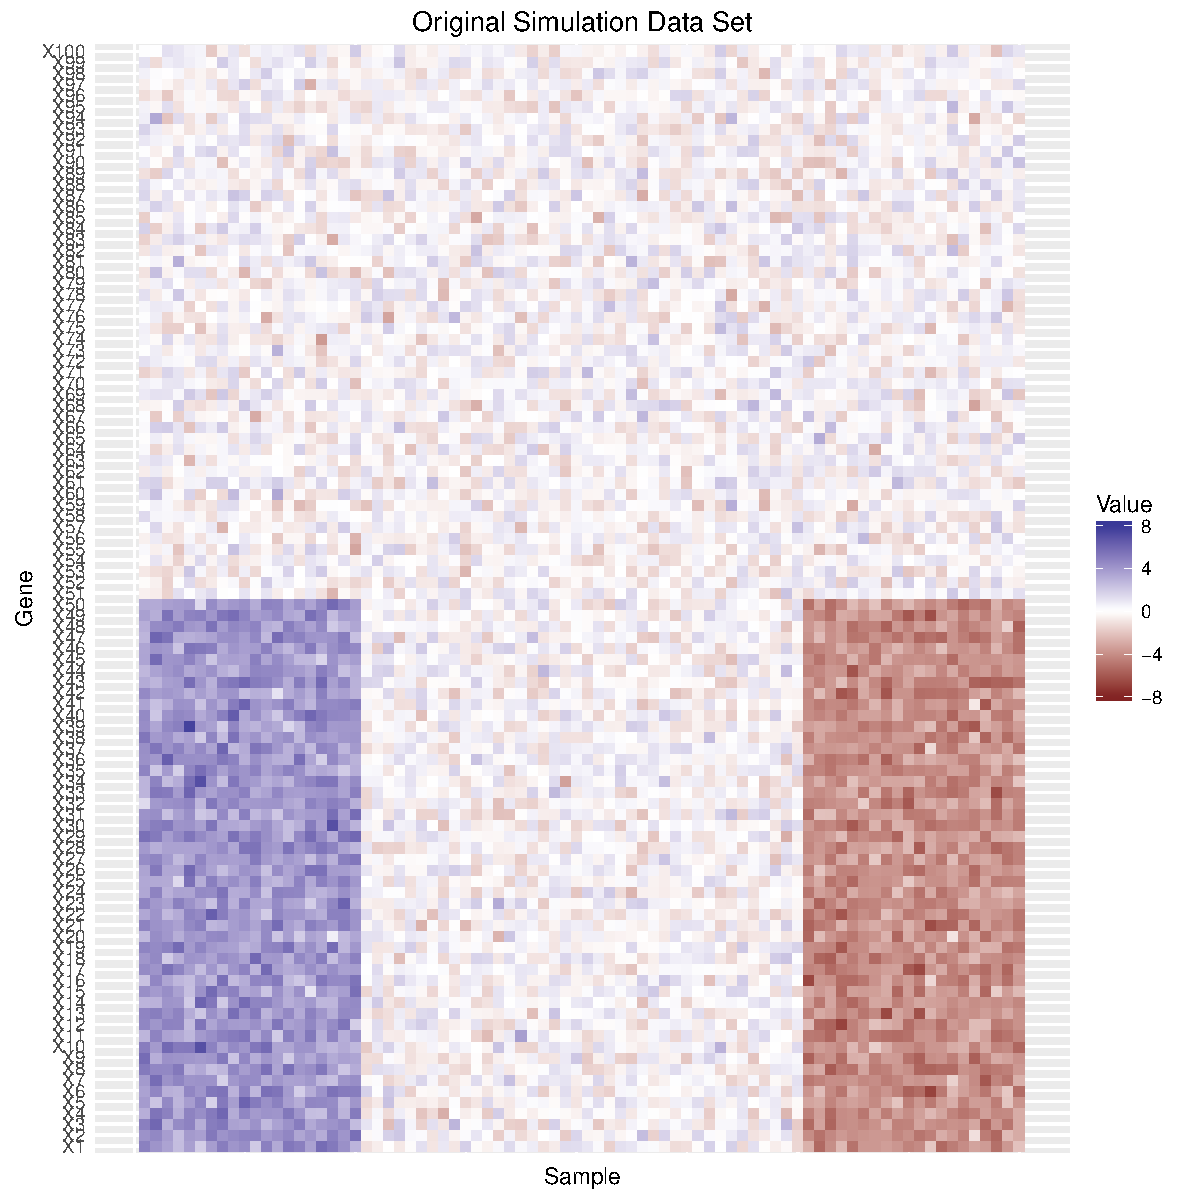
\includegraphics[width = \textwidth]{figures/simulate4.pdf}
        \caption{Original Simulation Data Set in the Case 1}
    \end{subfigure}% 
~
    \begin{subfigure}[b]{0.3\textwidth}
        \centering
        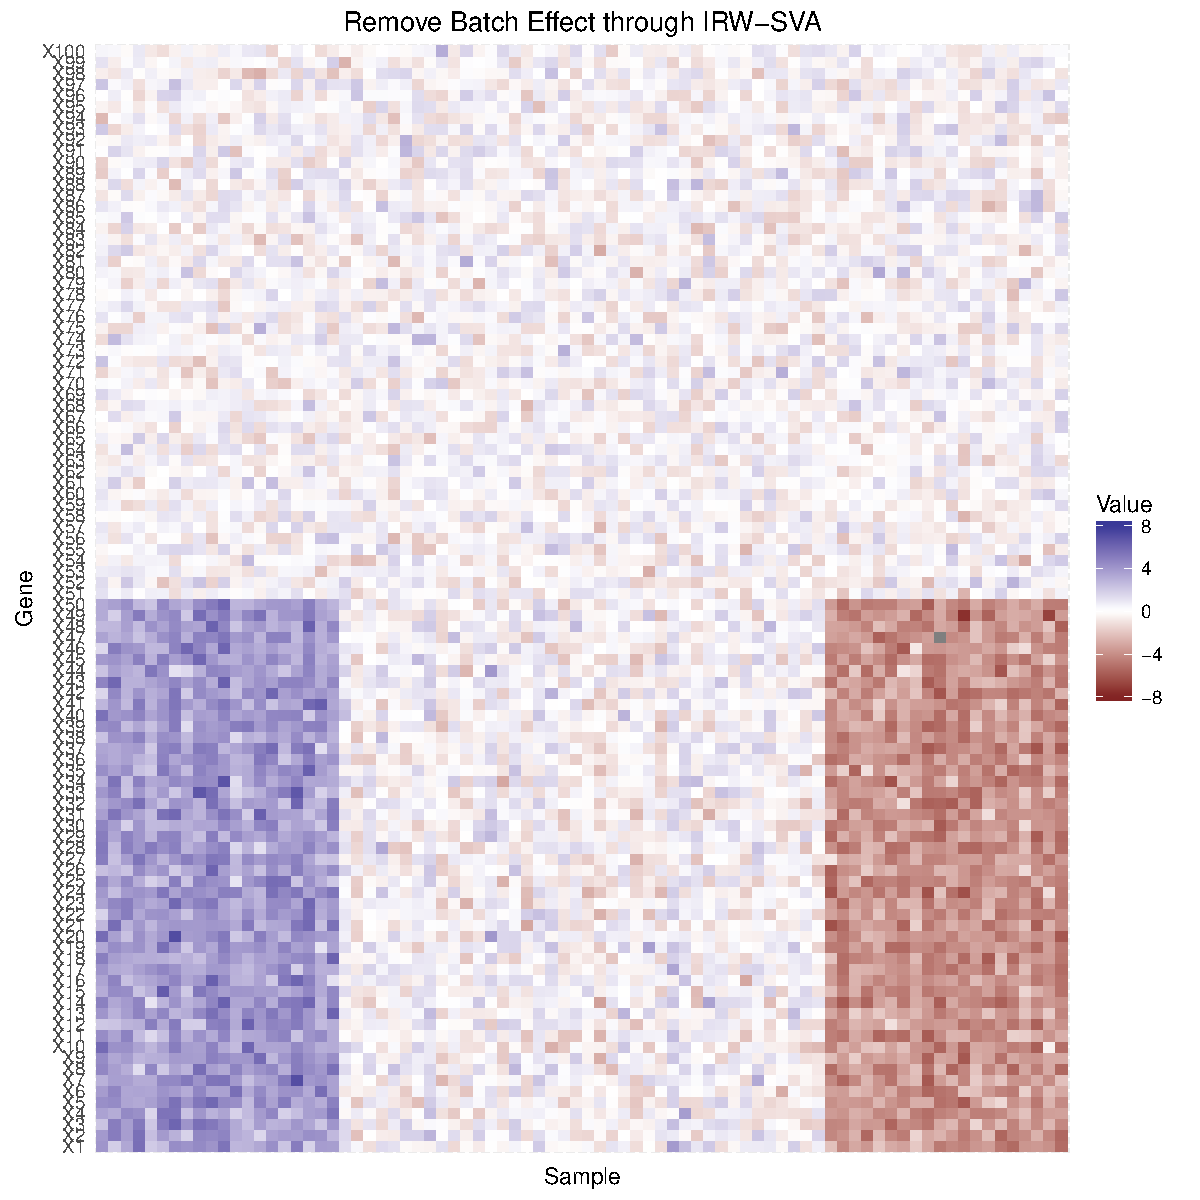
\includegraphics[width = \textwidth]{figures/sva4.pdf}
        \caption{Remove Batch Effect through IRW-SVA}
    \end{subfigure}  %
~
    \begin{subfigure}[b]{0.3\textwidth}
        \centering
        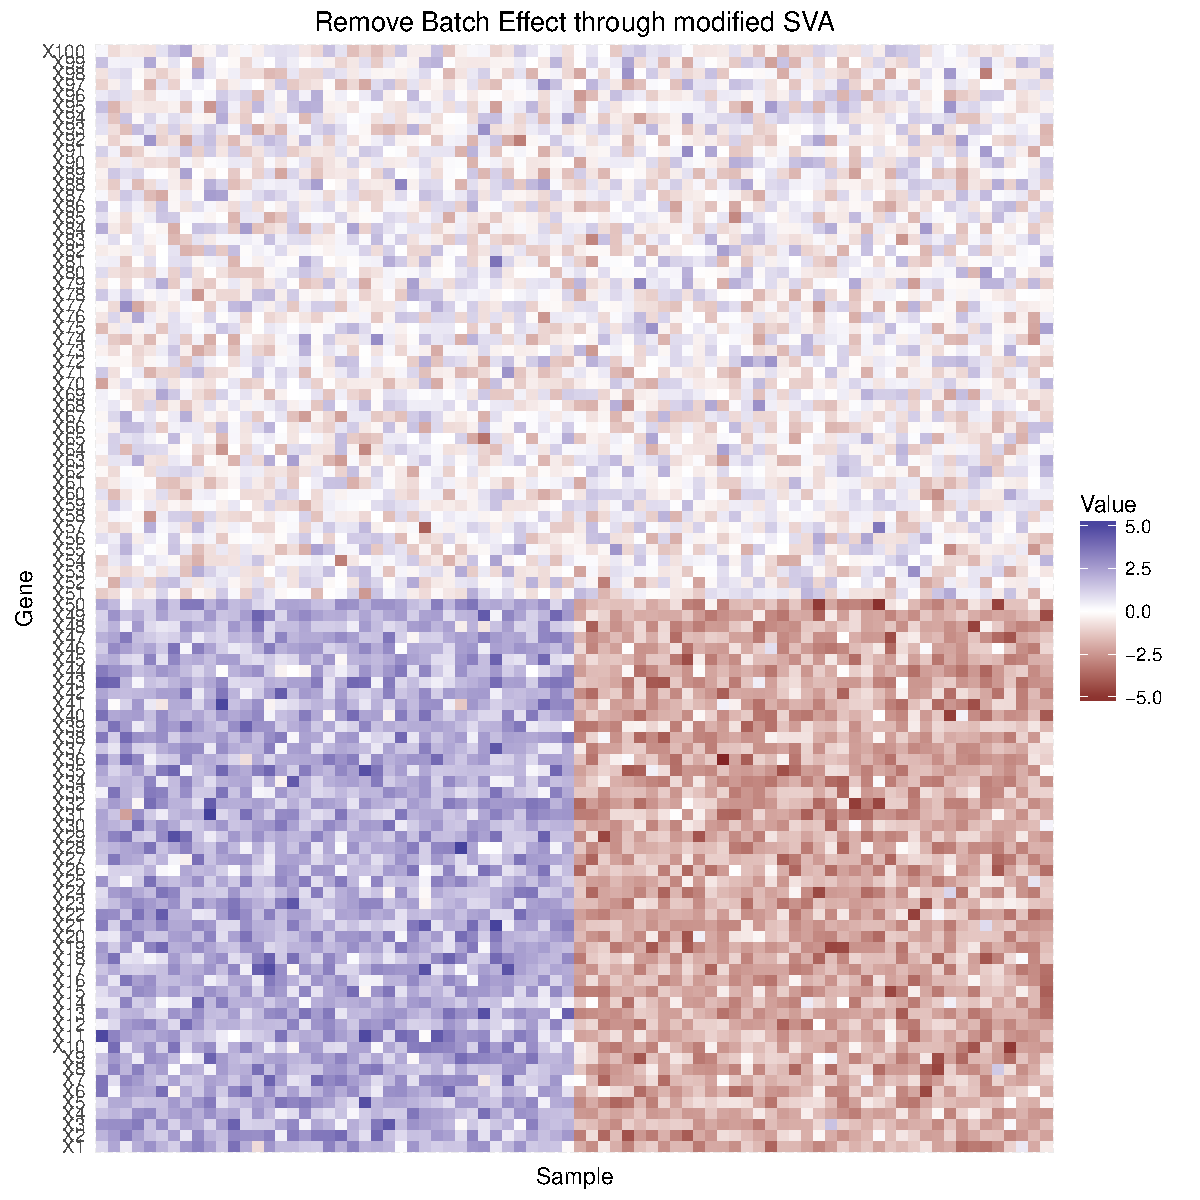
\includegraphics[width = \textwidth]{figures/new_sva4.pdf}
        \caption{Remove Batch Effect through modified SVA}
    \end{subfigure}    
    \caption{Remove Batch Effect Through Different Approaches of SVA in the Case 1}
\end{figure}



\begin{figure}[h!]
    \centering
    \begin{subfigure}[t]{0.46\textwidth}
    \centering
    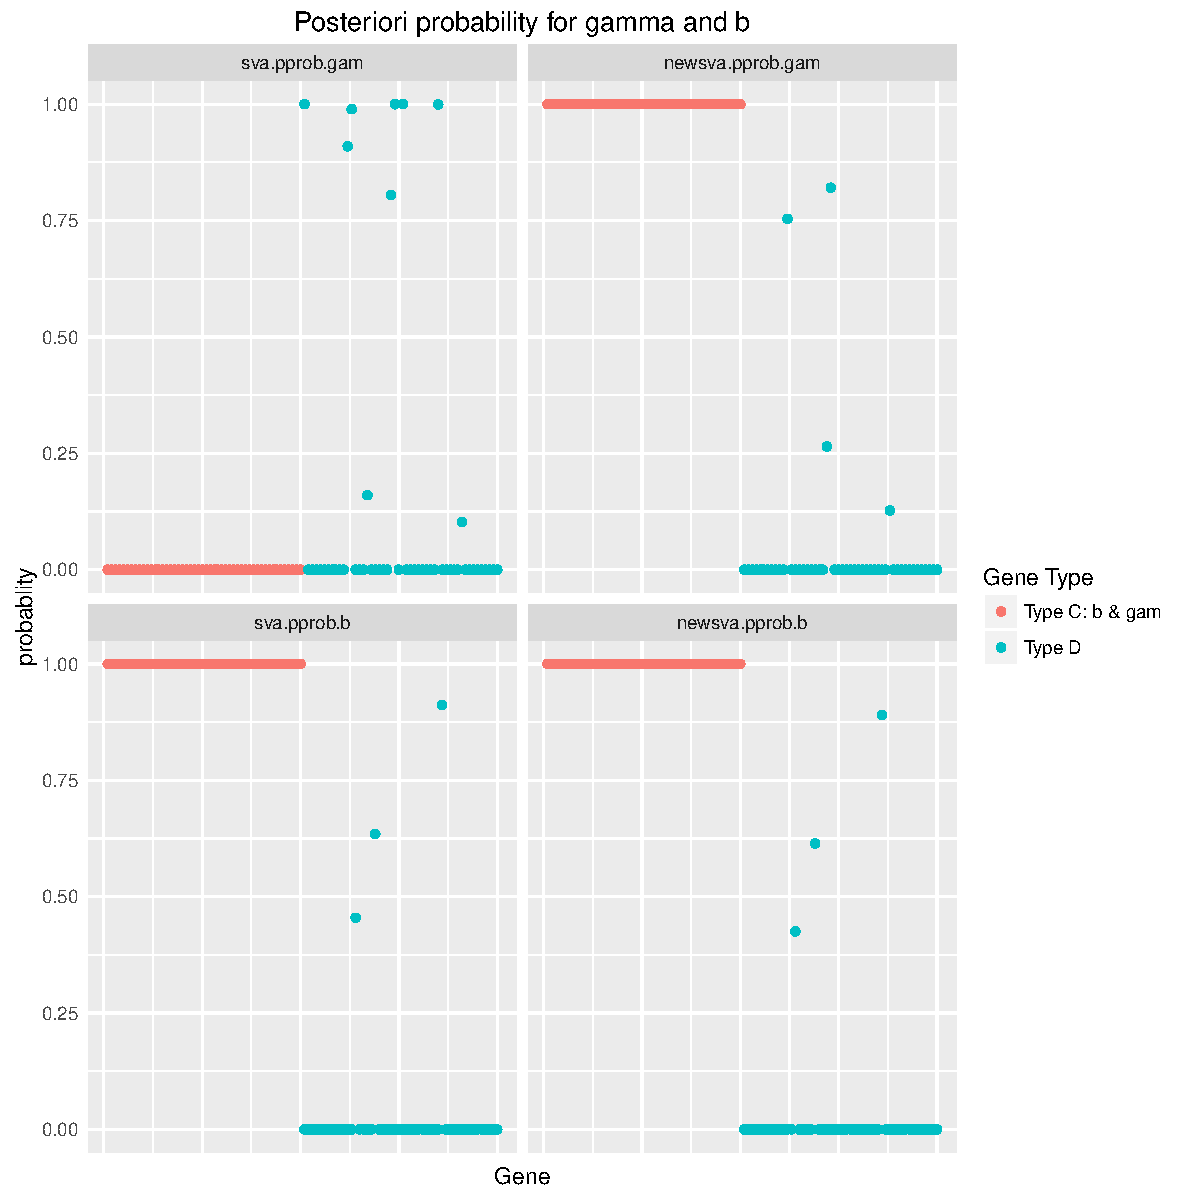
\includegraphics[width = \textwidth]{figures/pprop4.pdf}
    \caption{Posterior probability of $\mathbb{P}(b \neq 0 | X, S, \hat{G})$ and $\mathbb{P}(\gamma \neq 0 | X, S, \hat{G})$}
    \end{subfigure}
~    
    \begin{subfigure}[t]{0.46\textwidth}
    \centering
    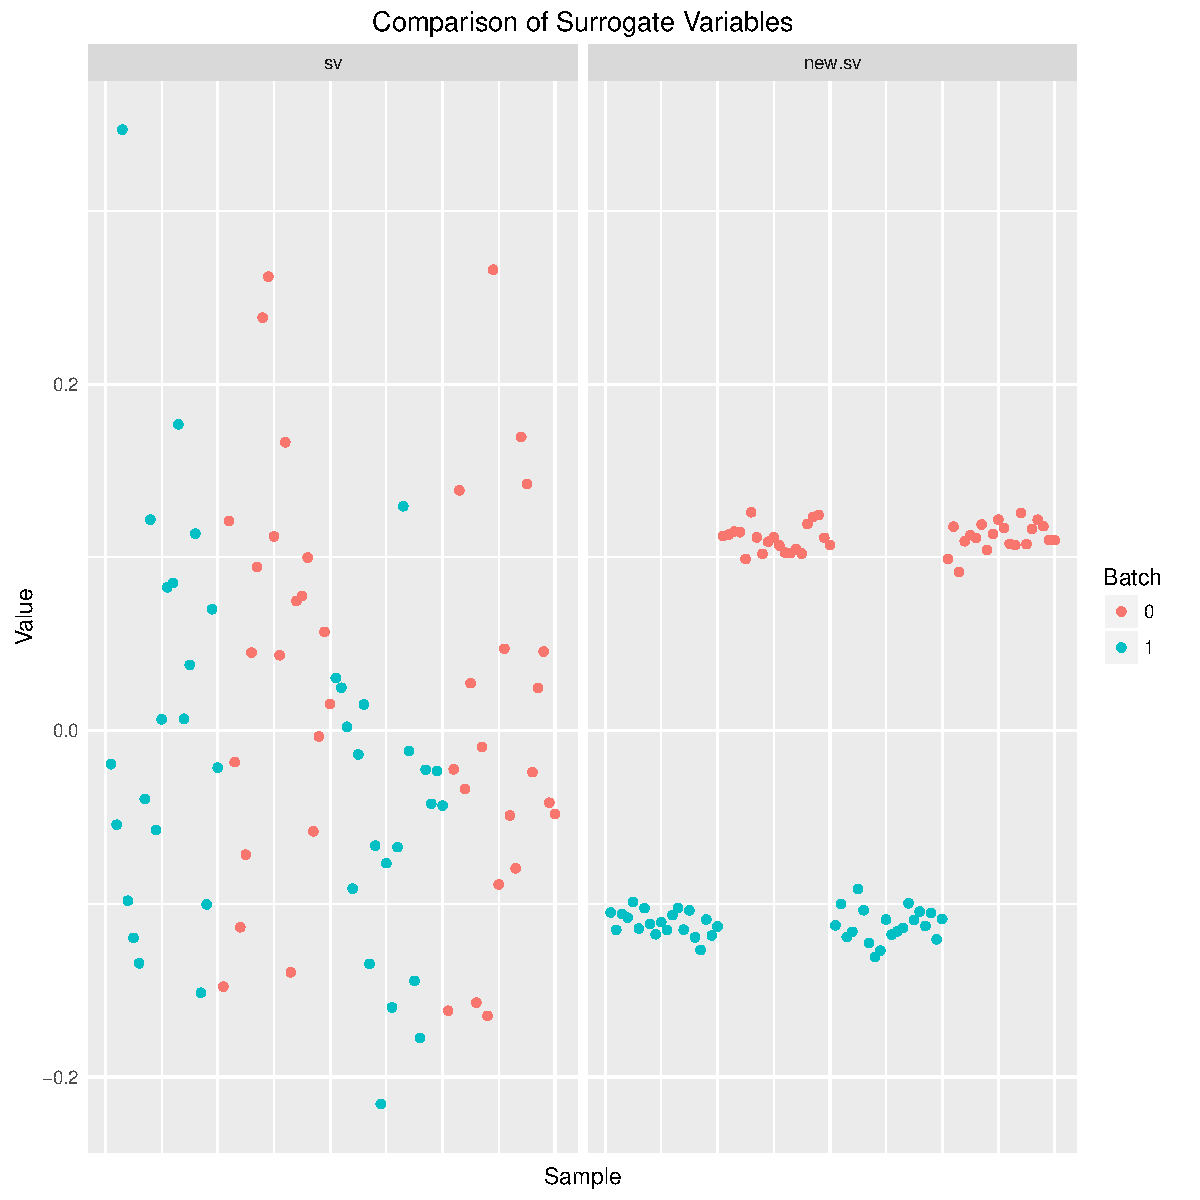
\includegraphics[width = \textwidth]{figures/vector4.pdf}
    \caption{Comparison of Surrogate Variables}
    \end{subfigure}
    \caption{Visualize The Analysis Through Sample Space And Gene Space in the Case 1}
\end{figure}


\newpage

\subsection{Case 2: The simulation data set contains all four types of genes.}

In the Case 2, IRW-SVA and modified SVA both work pretty well and they produce similar surrogate variable.

\begin{figure}[h!]
    \centering
    \begin{subfigure}[b]{0.3\textwidth}
        \centering
        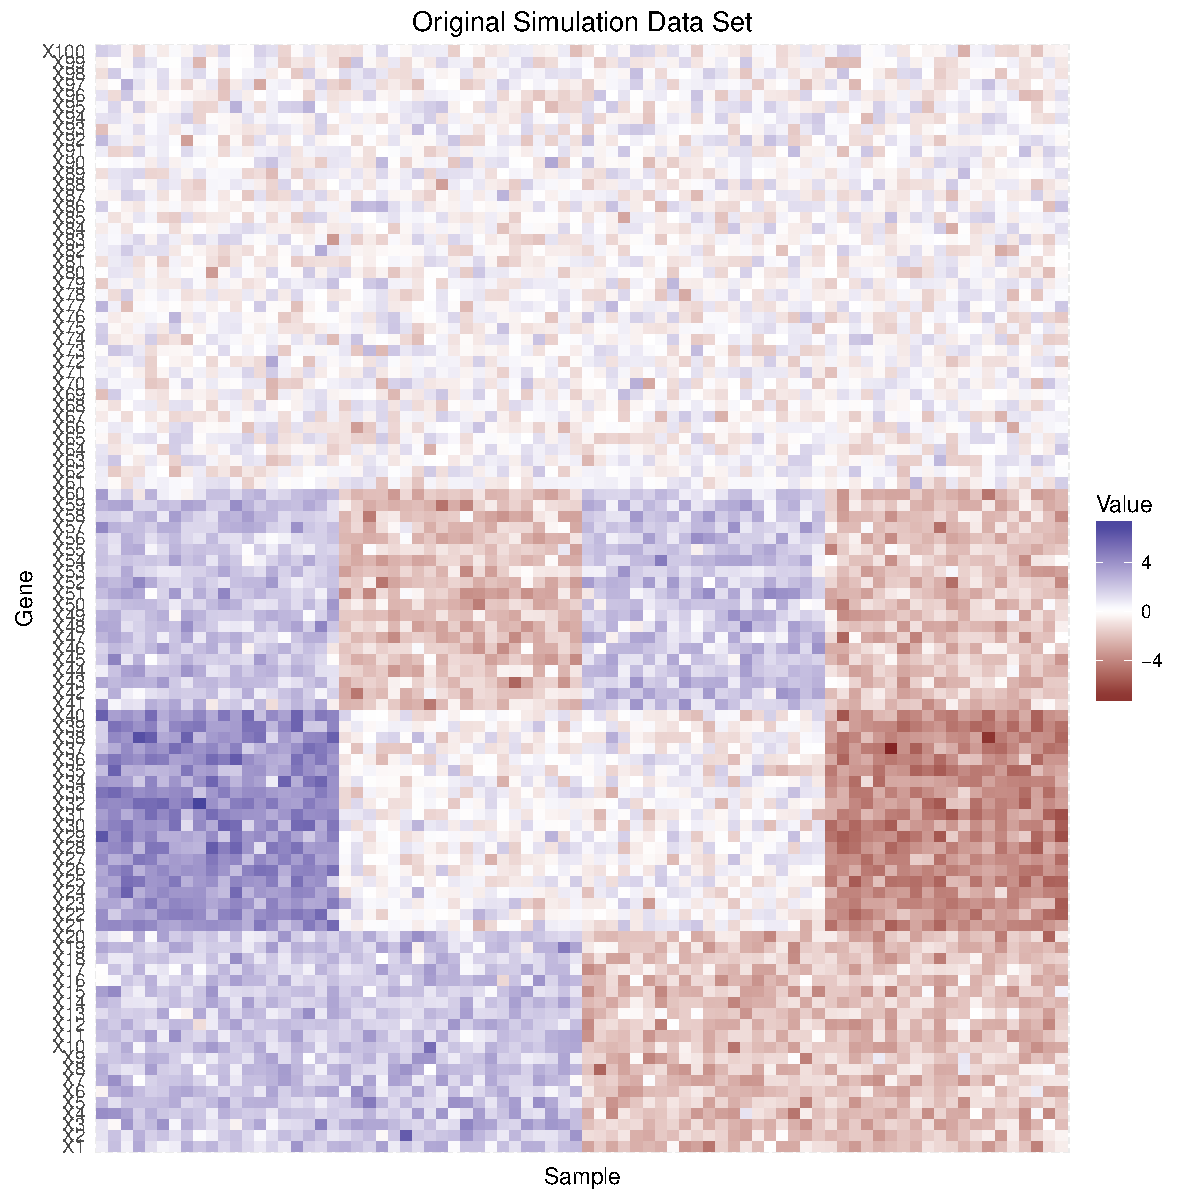
\includegraphics[width = \textwidth]{figures/simulate0.pdf}
        \caption{Original Simulation Data Set in the Case 2}
    \end{subfigure}% 
~
    \begin{subfigure}[b]{0.3\textwidth}
        \centering
        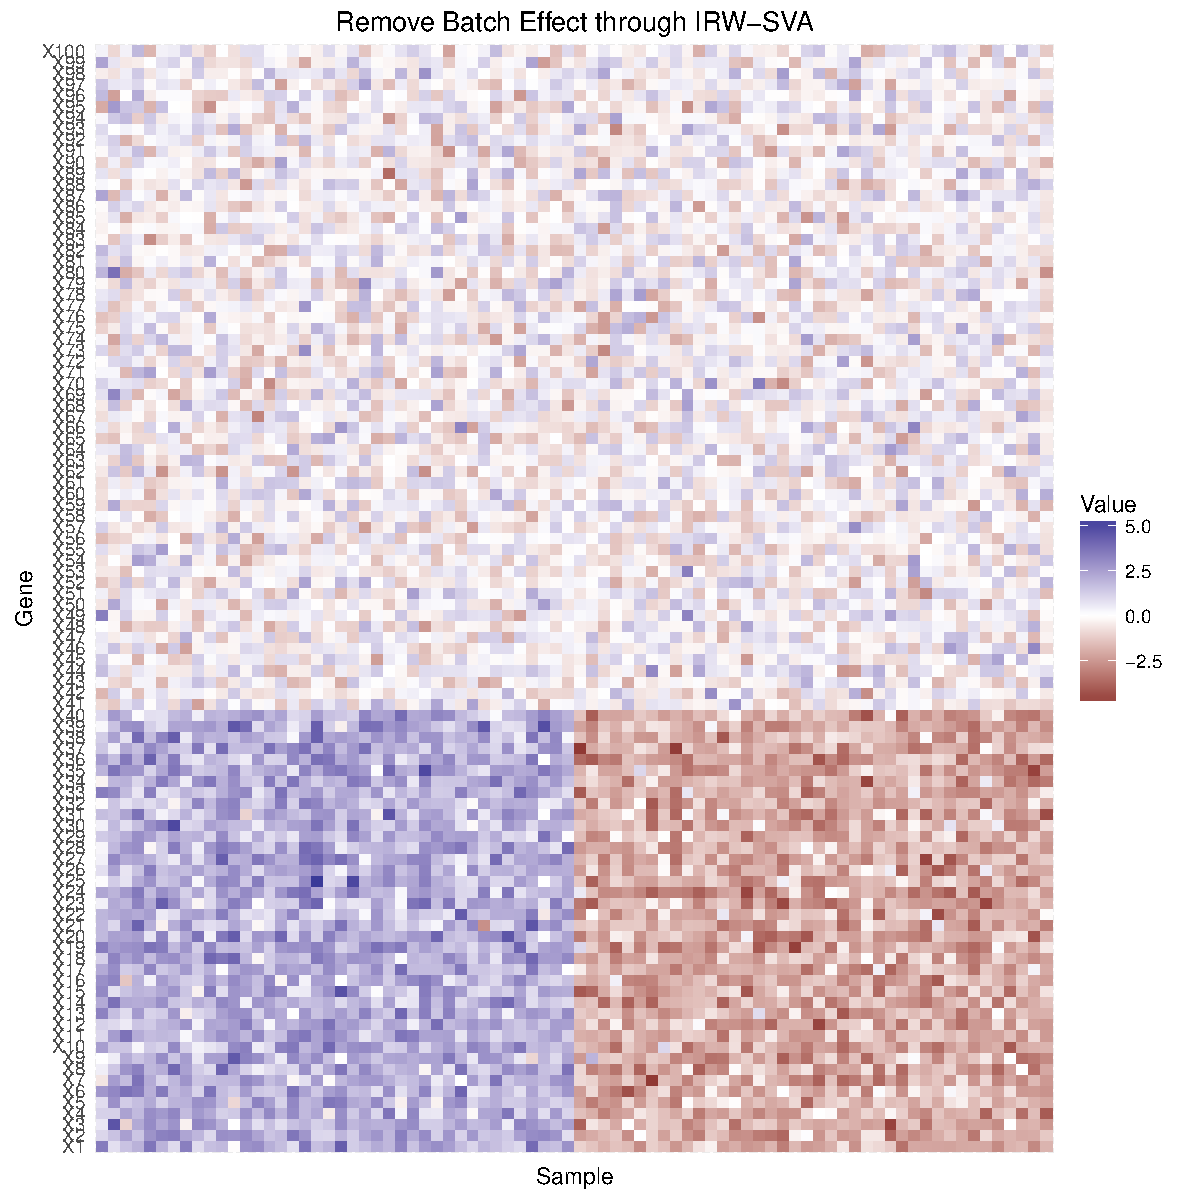
\includegraphics[width = \textwidth]{figures/sva0.pdf}
        \caption{Remove Batch Effect through IRW-SVA}
    \end{subfigure}  %
~
    \begin{subfigure}[b]{0.3\textwidth}
        \centering
        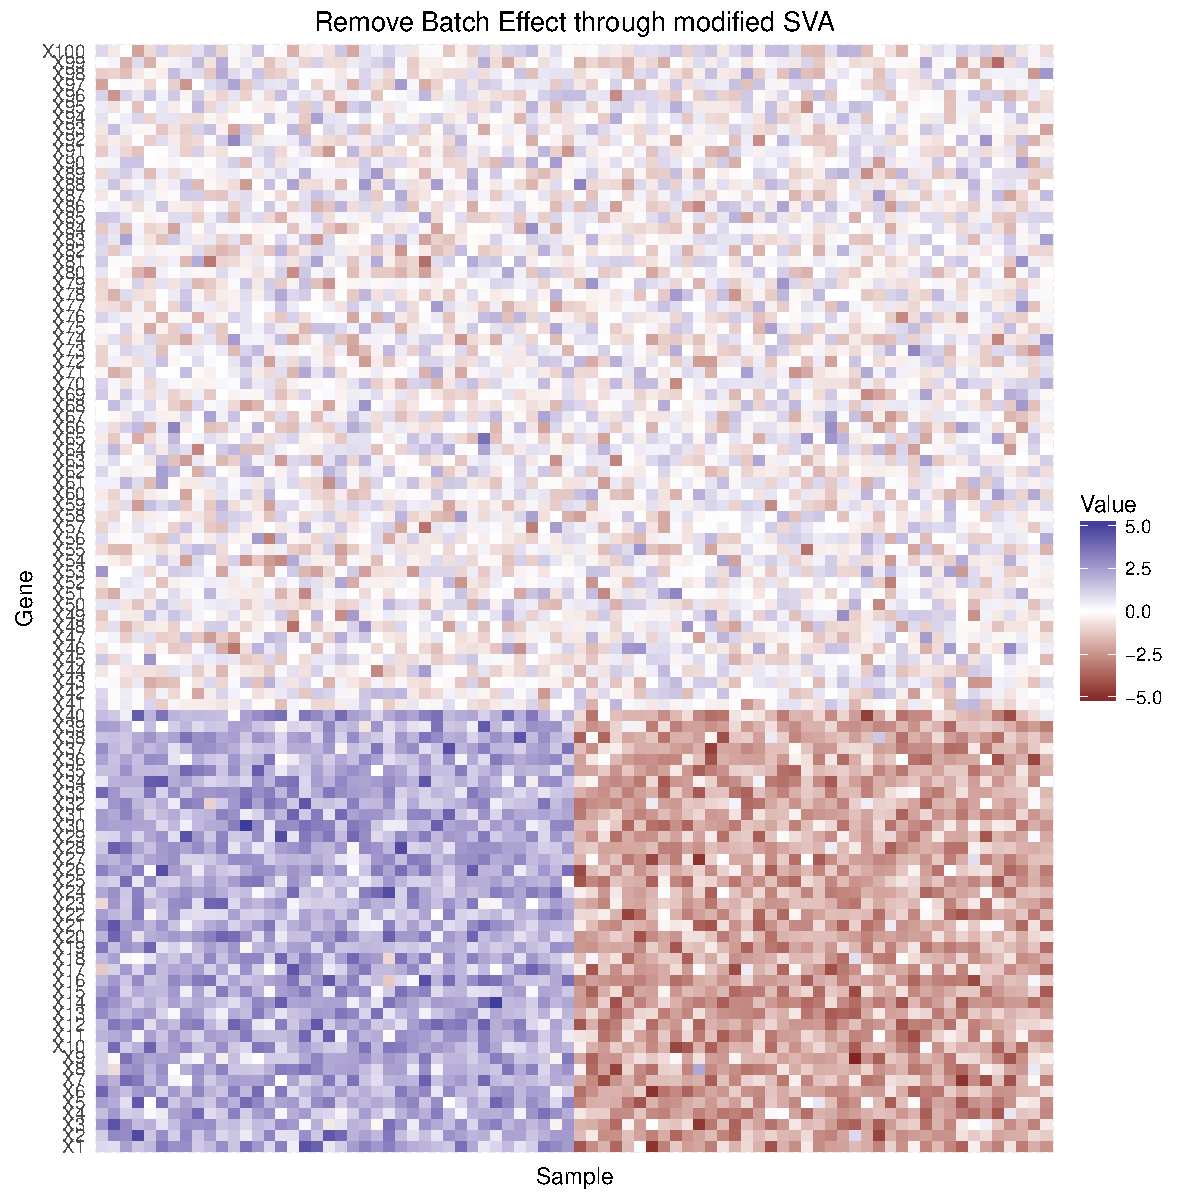
\includegraphics[width = \textwidth]{figures/new_sva0.pdf}
        \caption{Remove Batch Effect through modified SVA}
    \end{subfigure}    
    \caption{Remove Batch Effect Through Different Approaches of SVA in the Case 2}
\end{figure}


\begin{figure}[h!]
    \centering
    \begin{subfigure}[t]{0.46\textwidth}
    \centering
    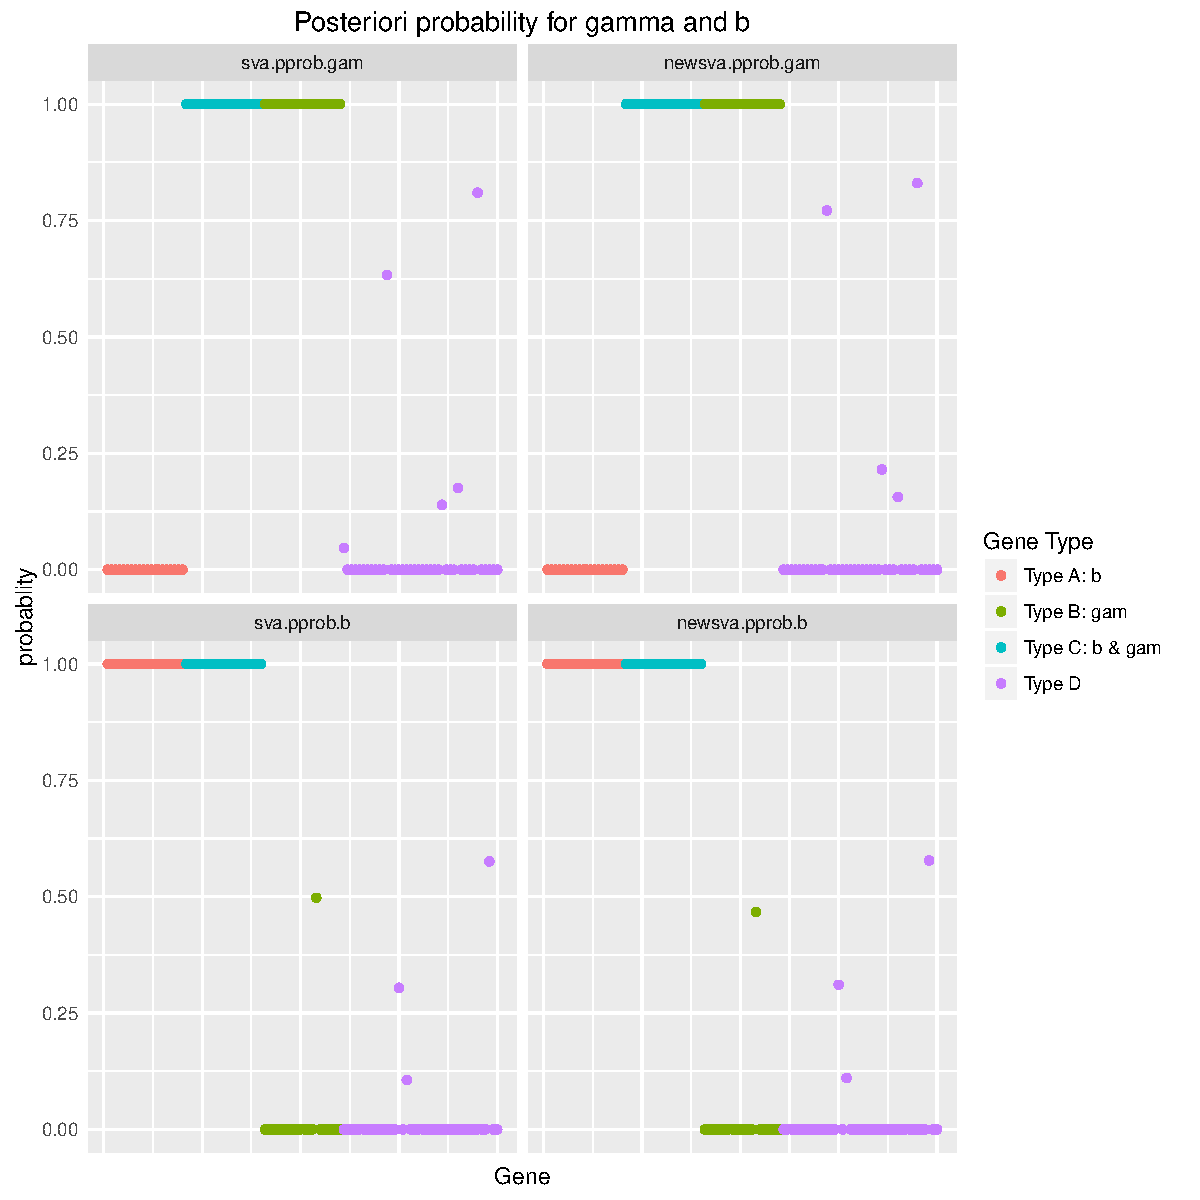
\includegraphics[width = \textwidth]{figures/pprop0.pdf}
    \caption{Posterior probability of $\mathbb{P}(b \neq 0 | X, S, \hat{G})$ and $\mathbb{P}(\gamma \neq 0 | X, S, \hat{G})$}
    \end{subfigure}
~    
    \begin{subfigure}[t]{0.46\textwidth}
    \centering
    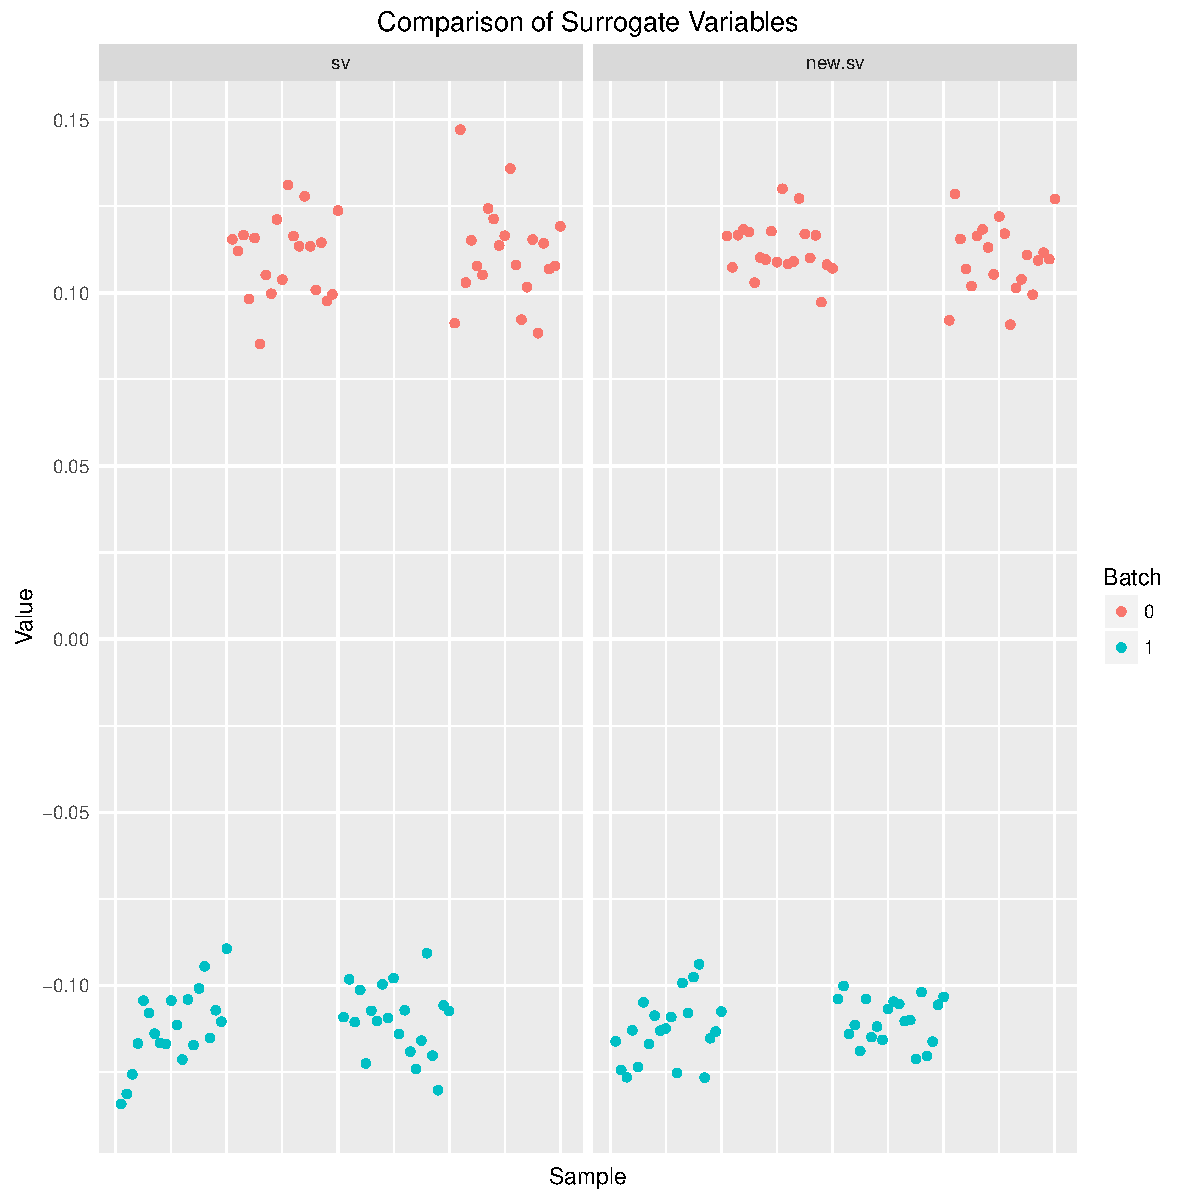
\includegraphics[width = \textwidth]{figures/vector0.pdf}
    \caption{Comparison of Surrogate Variables}
    \end{subfigure}
    \caption{Visualize The Analysis Through Sample Space And Gene Space in the Case 2}
\end{figure}

\newpage


\bibliographystyle{plain}
\bibliography{svabib}

\end{document}